\chapter{Аналитическая часть}
\section{Кодирование}
Кодирование информации --- отображение данных на кодовые слова. Обычно в процессе кодирования информация преобразуется из формы, удобной для непосредственного использования, в форму, удобную для передачи, хранения или автоматической обработки. Кодирование используется для адаптации данных к среде или технологии, в которой они будут использоваться.

\section{Алгоритм Хаффмана}
Алгоритм Хаффмана — это эффективный метод сжатия данных, который используется для кодирования символов с помощью префиксных кодов(система кодирования, в которой никакой код не является началом (или префиксом) другого кода). Символы, встречающиеся чаще, кодируются более короткими последовательностями битов, а менее частые символы — более длинными. Это позволяет минимизировать общее количество битов, используемых для хранения данных.

{\centering
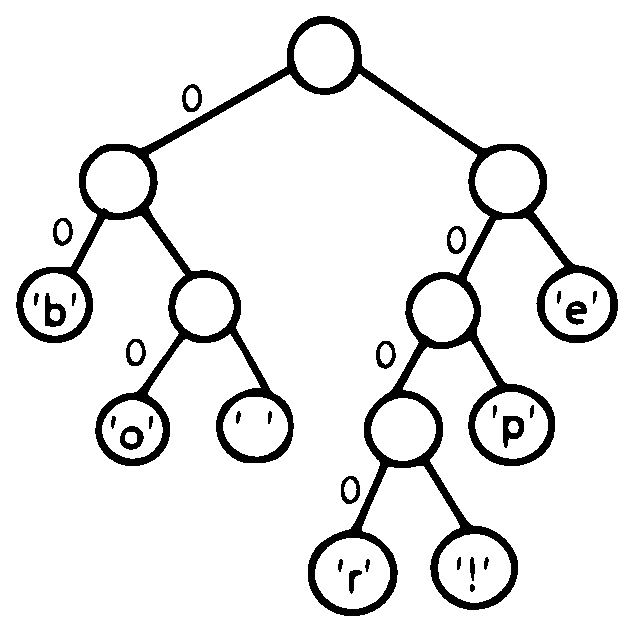
\includegraphics[scale = 0.6]{huf.eps}
\captionof{figure}{Пример кодирования}
}
\clearpage
